% Copyright (c) 2017 Peter A. Audano III
% GNU Free Documentation License Version 1.3 or later
% See the file COPYING.DOC for copying conditions.

\documentclass[a4paper]{article}

\usepackage[parfill]{parskip}  % Block paragraphs
\usepackage[margin=2.5cm]{geometry}  % Set margins
\usepackage{float}  % For H float placement
\usepackage{graphicx}  % Graphics

\usepackage[bottom]{footmisc}  % Footer
\usepackage{longtable}  % Multi-page table

% Set graphics extension
\DeclareGraphicsExtensions{.eps}

% Set bibliography style
\usepackage[sort&compress,comma]{natbib}  % Refereces and citations
\bibliographystyle{abbrvnat}  % Bibliography style

% Other style
\def\arraystretch{1.5}  % Pad tables

% Custom commands
\newcommand{\ddash}{{-}{-}}

\newcommand{\rsec}[1]{\textbf{Section~\ref{#1}}}     % Reference a section
\newcommand{\rfig}[1]{\textbf{Fig.~\ref{#1}}}        % Reference a figure
\newcommand{\rfigpart}[2]{\textbf{Fig.~\ref{#1}#2}}  % Reference a figure and part
\newcommand{\rtab}[1]{\textbf{Table~\ref{#1}}}       % Reference a table
\newcommand{\reqn}[1]{\textbf{Eqn.~\ref{#1}}}        % Reference an equation
\newcommand{\figpart}[1]{(\textbf{#1})}              % Annotate a figure part within the caption

% Date and title
\title{Kestrel Manual\\v1.0.0}
\date{}

%%%%%%%%%%%%%%%%%%%%%%
%%% Begin Document %%%
%%%%%%%%%%%%%%%%%%%%%%
\begin{document}

%%% Title %%%
\maketitle{}

%%% TOC %%%
\tableofcontents{}
\clearpage

%%% Section: Introduction %%%
% Copyright (c) 2017 Peter A. Audano III
% GNU Free Documentation License Version 1.3 or later
% See the file COPYING.DOC for copying conditions.

\section{Introduction}
\label{sec.intro}

\subsection{About Kestrel}
\label{sec.intro.aboutkestrel}

Kestrel is an alignment-free reference-guided variant caller. Given a reference sequence and sequence reads from an isolate, Kestrel identifies variations between the reference and the isolate. Most reference sequences are contained in one or more FASTA files, and they are long assembled representations of an organisms genome. Sequence reads if an individual, or isolate, are typically contained in one or more FASTQ files.

Kestrel can identify both single nucleotide polymorphism (SNP) and insertion/deletion (indel) variants without relying on sequence reads. Most variant-calling software reads alignments generated by other tools, such as BWA or bowtie. Kestrel reads directly from the FASTQ files and skips the genome alignment step. Although it uses some algorithms based on alignments, Kestrel is alignment-free because it never attempts to align the sequence reads to the reference.

The approach Kestrel takes is to first convert the sequence reads to k-mers, which are short overlapping fragments of a given length ($k$). For example, the 4-mers in ``AACCGG'' are ``AACC'', ``ACCG'', and ``CCGG''. By default, Kestrel uses a k-mer size of 31. Because it can communicate directly with KAnalyze, Kestrel can transform the sequence reads very quickly and begin the variant-calling process.

Kestrel has several advantages over traditional alignment-guided variant callers. In some cases, it may be faster because good alignments can take a long time build. Most importantly, it can process variant-dense regions were alignments fail, and it can identify arbitrarily large insertions.

When alignment techniques work correctly, they can produce more statistically-significant results. For Kestrel to function without relying on alignments, some of the original context is lost. For example, alignments can be improved with paired-end reads, but the paired-end context is lost in k-mer space. We recommend using Kestrel as a fast first-pass variant caller or in circumstances where alignments fail or where large insertions are suspected. In some pipelines, both alignment-guided and alignment-free approaches may be used together to find all possible variants.

\clearpage

%%% Section: Command Line Usage %%
% Copyright (c) 2017 Peter A. Audano III
% GNU Free Documentation License Version 1.3 or later
% See the file COPYING.DOC for copying conditions.

% Define table widths
\newcommand{\optwidth}{0.15\textwidth}
\newcommand{\argwidth}{0.20\textwidth}
\newcommand{\dscwidth}{0.50\textwidth}
\newcommand{\defwidth}{0.15\textwidth}

% Define table parboxes
\newcommand{\optbox}[1]{\parbox[t][][t]{\optwidth}{#1}\vspace{0.25em}}
\newcommand{\argbox}[1]{\parbox{\argwidth}{#1}}
\newcommand{\dscbox}[1]{\parbox{\dscwidth}{#1}}
\newcommand{\defbox}[1]{\parbox{\defwidth}{#1}}




\section{Command Line Usage}
\label{sec.cmdline}

Java 1.7 (aka Java 7) must be installed in order to run any commands in this section. Run \texttt{java -version} to see your version of Java. If you do not see ``java 1.7.0'' or a later version, Java must be updated before continuing.


%%%%%%%%%%%%%%%%%%%%
%%% Java Command %%%
%%%%%%%%%%%%%%%%%%%%
\subsection{Java Command}
\label{sec.cmdline.javacommand}

General form:\\
\texttt{java -jar -Xmx4G kestrel.jar <arguments ...>}

This allocates 4 GB of RAM (-Xmx4G).

If memory does not need to be tuned, the `kestrel` script may be run.

Do not separate `kestrel.jar` from the other JAR files. They must be in the same directory or Kestrel will not be able to find libraries it depends on, such as KAnalyze. You may create a symbolic link to `kestrel` from any directory.


%%%%%%%%%%%%%%%%%%%%%
%%% Example Usage %%%
%%%%%%%%%%%%%%%%%%%%%
\subsection{Example Usage}
\label{sec.cmdline.example}


%%% Example Usage %%%
\subsubsection{Example Usage}
\label{sec.cmdline.count.egusage}

\texttt{java -jar kestrel.jar count -r ref.fasta sample\_1.fastq sample\_2.fastq}\\
\hspace*{1cm}Reads reference sequences from ref.fasta and calls variants from the two FASTQ files as one sample.

\texttt{java -jar kestrel.jar count -r ref.fasta -i regions.bed sample\_1.fastq sample\_2.fastq}\\
\hspace*{1cm}Reads reference sequences from ref.fasta, extracts regions from the reference sequences in regions.bed, and calls variants from the two FASTQ files as one sample.


%%%%%%%%%%%%%%%%%%%%%%%
%%% Command options %%%
%%%%%%%%%%%%%%%%%%%%%%%
\subsection{Command options}
\label{sec.cmdline.opts}


\subsubsection{Getting Help}
\label{sec.cmdline.opts.help}

\begin{small}
	\begin{longtable}{|p{\optwidth}|p{\argwidth}|p{\dscwidth}|p{\defwidth}|}
		\hline
		
		% Header
		\textbf{Option} & \textbf{Argument} & \textbf{Description} & \textbf{Default} \\ \hline
	
		% Help
		\optbox{\sopt{h}\\\lopt{help}} & [TOPIC] &
		Get help on the command line. If TOPIC is not supplied, general command line usage and all options are printed. Print help on a specific topic if TOPIC is given. See -htopics (or \ddash{}help=topics) for a list of topics and -hcite for information about how to cite Kestrel.
		&
		\\ \hline
		
	\end{longtable}
\end{small}


\subsubsection{Input and Output}
\label{sec.cmdline.opts.io}

\begin{small}
	\begin{longtable}{|p{\optwidth}|p{\argwidth}|p{\dscwidth}|p{\defwidth}|}
		\hline
		
		% Header
		\textbf{Option} & \textbf{Argument} & \textbf{Description} & \textbf{Default} \\ \hline
		
		% Input format
		\optbox{\sopt{f}\\\lopt{format}} & FORMAT &
		Specify the format of input sequence files. Built-in readers are ``fastq'', ''fasta'', ``fastqgz'', ``fastagz'' for FASTQ and FASTA files and gzipped versions of them, and ``ikc'' for indexed k-mer count files (a KAnalyze format). The default, ``auto'', will attempt to determine the file type by its name. This option applies to all input files that follow it on the command line.
		& auto
		\\ \hline
		
		% Output file name
		\optbox{\sopt{o}\\\lopt{out}} & FILE &
		Name of the file where output should be directed.
		&
		\\ \hline
		
		% Stdout
		\lopt{stdout} & &
		Send output to the screen, STDOUT.
		& TRUE
		\\ \hline
		
		% Output format
		\optbox{\sopt{m}\\\lopt{outfmt}} & FORMAT &
		Format of the output. Built-in formats are ``vcf'', ``table'' for a tab-delimited table, and ``txt'' for readable text output.
		& vcf
		\\ \hline
		
		% Haplotype output
		\optbox{\sopt{p}\\\lopt{hapout}} & FILE &
		Set aligned haplotypes to an output file. If this option is not specified, haplotypes are not written.
		&
		\\ \hline
		
		% Haplotype format
		\lopt{hapfmt} & FORMAT &
		If haplotype output is enabled, then this is the format of the output file. The default, ``sam'', writes the aligned haplotypes relative to the reference sequence.
		& sam
		\\ \hline
		
		% Log file name
		\lopt{logfile} & FILE &
		Specify the name of a log file.
		&
		\\ \hline
		
		% Log to STDOUT
		\lopt{logstdout} & &
		Send log messages to STDOUT.
		&
		\\ \hline
		
		% Log to STDERR
		\lopt{logstderr} & &
		Send log messages to STDERR.
		& TRUE
		\\ \hline
		
		% Log level
		\lopt{loglevel} & LEVEL &
		Set the logging level. Valid log levels are ``ALL'', ``TRACE'', ``DEBUG'', ``INFO'', ``WARN'', ``ERROR'', and ``OFF''.
		& OFF
		\\ \hline
		
		% Files per sample
		\lopt{filespersample} & N &
		Automatically divide input files into discrete samples by the number of samples. This may be useful for loading many samples by listing them on the command-line. For example, to load paired-end reads in multiple samples, set this value to ``2''. Note that Kestrel does not associate files by their name, so related files must be grouped together in the order they are listed. The default, $0$, loads all files as a single sample.
		& 0
		\\ \hline
		
		% Sample set
		\optbox{\sopt{s}\\\lopt{sample}} & [NAME] &
		All input files on the command line following this option are grouped into a single sample with name NAME. If NAME is not specified, then the sample name is derived from the first input file in the sample set. If \ddash{}filespersample was specified, it is undone and all samples go into this sample set. If \ddash{}filespersample is specified at some point after this option, it takes precedence and splits files into samples.
		&
		\\ \hline
		
		% Reference
		\optbox{\sopt{r}\\\lopt{ref}} & FILE &
		Specifies the name of the FASTA file containing the reference sequences variants are called against. This option may be used multiple times, and FASTA files may contain any number of records. All FASTA Records must have a unique description.
		&
		\\ \hline
		
		% K-mer size
		\optbox{\sopt{k}\\\lopt{ksize}} & KSIZE &
		Specify the size of k-mers sequence data is transformed to.
		& 31
		\\ \hline
		
		% Library
		\lopt{lib} & FILE &
		Load an external library containing extensions for Kestrel, such as a custom output format. FILE may be a JAR file or a directory containing Java class files.
		&
		\\ \hline
		
		% Library URL
		\lopt{liburl} & URL &
		Load a library containing extensions for Kestrel. The library is specified as a URL string, and it can be any URL facility that Java can recognize, locate, and load.
		&
		\\ \hline
		
		% Charset
		\lopt{charset} & CHARSET &
		Character set encoding of input files. This option specifies the character set of all files following it. The default, ``UTF-8'', properly handles ASCII files, which is a safe assumption for most files. Latin-1 files with values greater than 127 will not be properly parsed.
		& UTF-8
		\\ \hline
		
		% Sequence filter
		\optbox{\lopt{seqfilter}\\\lopt{quality}} & SPEC &
		Filter sequences as they are read and before k-mers are extracted from them. Some sequence readers can filter or alter reads at runtime. The most common filter is a quality filter where low-quality bases are removed. The filter specification is a filter name followed by a colon (:) and arguments to the filter. If a filter name is not specified, then the ``sanger'' quality filter is assumed. For example, ``sanger:10'' and ``10'' will filter k-mers with any base quality score less than 10. The sequence filter specification is set for all files appearing on the command-line after this option. To turn off filtering once it has been set, files following \ddash{}noseqfilter will have no filter specification.
		&
		\\ \hline
		
		% No sequence filter
		\lopt{noseqfilter} & &
		Turn off filters for input files following this option.
		&
		\\ \hline
		
		% Temp file location
		\lopt{temploc} & DIR &
		Name of the directory where KAnalyze stores temporary files when processing sequence data for Kestrel.
		& \parbox{2cm}{Current\\directory}
		\\ \hline
		
		% Minimum k-mer count
		\lopt{mincount} & COUNT &
		A k-mer with a frequency of this value or less is ignored. This keeps the IKC file to a reasonable size by reducing the number of erroneous k-mers from sequencing errors.
		& 5
		\\ \hline
		
		% Minimizer size
		\lopt{minsize} & &
		Minimizers group k-mers in the indexed k-mer count (IKC) file generated by Kestrel when reading sequences, and this parameter controls the size of the minimizer.
		& 15
		\\ \hline
		
		% Minimizer mask
		\lopt{minmask} & &
		K-mers over low-complexity loci may create large minimizer groups, and a minimizer mask may break up these groups.
		& 0x00000000
		\\ \hline
		
		% Count in memory
		\lopt{memcount} & &
		When sequence reads are input, this option will count them in memory instead of an IKC file.
		&
		\\ \hline
		
		% No count in memory
		\lopt{nomemcount} & &
		When sequence reads are input, generate an IKC file and query k-mer frequencies from it.
		& TRUE
		\\ \hline
		
		% Remove IKC
		\lopt{rmikc} & &
		Remove the indexed k-mer count (IKC) for each sample after kestrel runs.
		& TRUE
		\\ \hline
		
		% No remove IKC
		\lopt{normikc} & &
		Do not remove the indexed k-mer count (IKC) file for each sample.
		& TRUE
		\\ \hline
		
		% Count reverse k-mers
		\lopt{countrev} & &
		Count reverse complement k-mers in region statistics. This should be set for most sequencing protocols.
		& TRUE
		\\ \hline
		
		% No count reverse k-mers
		\lopt{nocountrev} & &
		Do not include the reverse complement of k-mers in read depth estimates. Only k-mers in reference orientation will be used.
		&
		\\ \hline
		
		% Read interval
		\optbox{\sopt{i}\\\lopt{interval}} & FILE &
		Reads a file of intervals defining the regions over the reference sequences where variants should be detected. If no intervals are specified, variants are detected over the full length of each reference sequence. The file type is determined by the file name, such as ``intervals.bed''.
		&
		\\ \hline
		
		% Flank length
		\lopt{flank} & LENGTH &
		When reading an interval from a reference, extract sequences beyond the boundaries of the interval to assist active region detection. Variants within the flanks are discarded.
		&
		$k \cdot 3.5$
		\\ \hline
		
		% Default flank length
		\lopt{autoflank} & &
		When calling variants with an interval file (a BED files that restricts calling to specific regions), extend active region detection beyond the region boundaries. Variants found outside regions are still discarded. This makes better calls for variants at the edge of the regions. The flank length is automatically chosen by the k-mer size if this option is not used.
		& $k \cdot 3.5$
		\\ \hline
		
		% By reference
		\lopt{byreference} & &
		If variant call regions were defined, variant call locations are relative to the reference sequence and not the region.
		& TRUE
		\\ \hline
		
		% By region
		\lopt{byregion} & &
		If variant call regions were defined, variant call locations are relative to each region instead of the reference sequence.
		&
		\\ \hline
		
		% Remove reference description
		\lopt{rmrefdesc} & &
		When set, remove the description from reference sequence names. The descirption is everything that occurs after the first whitespace character. FASTA files often have a sequence name and a long description separated by whitespace. This option ensures that the sequence name matches in the FASTA and an interval file, if used.
		& TRUE
		\\ \hline
		
		% Do not remove the reference description
		\lopt{normrefdesc} & &
		Use the full sequence name as it appears in the reference sequence file. FASTA files often include a description after the sequence name, and with this option, it becomes part of the full sequence name. If using an interval file, the full sequence name and description must match the sequence file.
		&
		\\ \hline
		
		% Reverse region
		\lopt{revregion} & &
		When set, reverse complement reference regions that occur on the negative strand, and all variant calls are relative to the reverse-complemented sequence. Only itervals defined with on the negative strand are altered.
		&
		\\ \hline
		
		% No reverse region
		\lopt{norevregion} & &
		When set, regions variants are called on are always in the same orientation as the reference sequence. The stranded-ness of defined intervals is ignored.
		& TRUE
		\\ \hline
		
	\end{longtable}
\end{small}

% End Input and Output


\subsection{Active Region Detection}
\label{sec.cmdline.opts.ardetect}

\begin{small}
	\begin{longtable}{|p{\optwidth}|p{\argwidth}|p{\dscwidth}|p{\defwidth}|}
		\hline
		
		% Header
		\textbf{Option} & \textbf{Argument} & \textbf{Description} & \textbf{Default} \\ \hline
		
		% Min count diff
		\lopt{mindiff} & DIFF &
		Set the minimum k-mer count difference for identifying active regions. The difference threshold determined by the difference quantile will never be less than this value.
		& 5
		\\ \hline
		
		% Difference quantile
		\lopt{diffq} & DIFFQ &
		If set to a value greater than 0.0, then the k-mer count difference between two k-mers that triggers an active region scan is found dynamically. The difference in k-mer counts between each pair of neighboring k-mers over an uncorrected reference region is found, and this quantile of is computed over those differences. The default value of 0.90 means that at most 10\% of the k-mer count differences will be high enough. If this computed value is less than the minimum k-mer count difference (\ddash{}mindiff), then that minimum is the difference threshold. This value may not be 1.0 or greater, and it may not be negative. If 0.0, the minimum count difference is always the minimum threshold (\ddash{}mindiff).
		& 0.90
		\\ \hline
		
		% Peak scan length
		\lopt{peakscan} & LENGTH &
		Reference regions with sequence homology in other regions of the genome may contain k-mers with artificially high frequencies from adding counts for k-mers that appear in those regions. This causes a peak in the k-mer frequencies over the reference, and it can trigger an erroneous active-region scan for variants. Kestrel will scan forward this number of k-mers looking for a peak in the k-mer frequencies. If the counts drop back down to the original range, the active region scan is stopped. This keeps Kestrel from erroneously searching large regions of the reference. Setting this value to 0 disables peak detection.
		& 7
		\\ \hline
		
		% Scan limit factor		
		\lopt{scanlimitfactor} & FACTOR &
		Set a limit on how long an active region may be. This is computed by multiplying the k-mer size by this factor and adding the maximum length of a gap. The computed limit will be adjusted so that active regions are at least large enough to capture a SNP in cases where the maximum gap length is 0. Setting this to a low value or ``min'' will set the limit so that it is just large enough to catch SNPs and deletions, but it will miss large deletions if another variant is within the k-mer size window. Setting this to a high value or ``max'' lifts the restrictions on active region lengths, and this may cause the program to take an excessive amount of time and memory trying to solve arbitrarily long active regions.
		& 5.0
		\\ \hline
		
		% Decay minimum
		\lopt{decaymin} & FACTOR &
		Set the minimum value (asymptotic lower bound) of the exponential decay function used in active region detection as a proportion of the anchor k-mer count. If this value is 0.0, k-mer count recovery threshold may decline to 1. If this value is 1.0, the decay function is not used and the detector falls back to finding a k-mer with a count within the difference threshold of the anchor k-mer count.
		& 0.55
		\\ \hline
		
		% Decay alpha
		\lopt{alpha} & ALPHA &
		Set the exponential decay alpha, which controls how quickly the recovery threshold declines to its minimum value (see \ddash{}decaymin) in an active region search. Alpha is defined as the rate of decay for every k bases. At k bases from the left anchor, the threshold will have declined to $\alpha \cdot$ range. At every k bases, the threshold will continue to decline at this rate ($\alpha^n \cdot$ range).
		& 0.80
		\\ \hline
		
		% Anchor both
		\lopt{anchorboth} & &
		Active regions may not go to the ends of the references. This reduces false-calls from noise, but it can miss variant calls near the ends.
		& TRUE
		\\ \hline
		
		% No anchor both
		\lopt{noanchorboth} & &
		Active regions ma go to the ends of the references. This may call variants near the ends, but it may also result in false calls.
		&
		\\ \hline
		
		% Amiguous regions
		\lopt{ambiregions}  & &
		Allow active regions that contain ambiguous bases.
		& TRUE
		\\ \hline
		
		% No ambiguous regions
		\lopt{noambigregions} & &
		Discard all active regions that contain at least one ambiguous base.
		&
		\\ \hline
		
	\end{longtable}
\end{small}

% End Active Region Detection


\subsection{Haplotype Reconstruction}
\label{sec.cmdline.opts.haplo}

\begin{small}
	\begin{longtable}{|p{\optwidth}|p{\argwidth}|p{\dscwidth}|p{\defwidth}|}
		\hline
		
		% Header
		\textbf{Option} & \textbf{Argument} & \textbf{Description} & \textbf{Default} \\ \hline
		
		% Alignment weight vector
		\optbox{\sopt{w}\\\lopt{weight}} & VECTOR &
		Set the alignment weights as a comma-separated list of values. The order of weights is match, mismatch, gap-open, gap-extend, and initial score. If values are blank or the list has fewer than 5 elements, the missing values are assigned their default weight. Each value is a floating-point number, and it may be represented in exponential form (e.g. 1.0e2) or as an integer in hexadecimal or octal format. Optionally, the list may be surrounded by parenthesis or braces (angle, square, or curly). If the initial score is empty or missing, it defaults to the k-mer size multiplied by the match score.
		& ``10, -10, -40, -4, 0''
		\\ \hline
		
		% Maximum align states
		\lopt{maxalignstates} & STATES &
		Set the maximum number of alignment states. When haplotype assembly branches into more than one possible sequence, the state of one is saved while another is built. When the maximum number of saved states reaches this value, the least likely one is discarded.
		& 15
		\\ \hline
		
		% Maximum haplotypes
		\lopt{maxhapstates} & STATES &
		Set the maximum number of haplotypes for an active region. Alignments can generate more than one haplotype, and with noisy sequence data or paralogues, many haplotypes may be found. This options limits the amount of memory that can be consumed in these cases.
		& 15
		\\ \hline
		
		% Maximum repeat count
		\lopt{maxrepeat} & COUNT &
		Set the maximum number of times k-mers may be repeated in active region construction. Repeated k-mers are cycles in the k-mer graph, and an assembly cannot proceed through such cycles unambiguously. The default value (0) is correct for most applications, but it may be increased to attempt assemblies through repetitive sequence. If this value is set above 0, then care must be taken when analyzing the output.
		& 0
		\\ \hline

	\end{longtable}
\end{small}

% End Haplotype Reconstruction


\subsection{Variant Calling}
\label{sec.cmdline.opts.haplo}

\begin{small}
	\begin{longtable}{|p{\optwidth}|p{\argwidth}|p{\dscwidth}|p{\defwidth}|}
		\hline
		
		% Header
		\textbf{Option} & \textbf{Argument} & \textbf{Description} & \textbf{Default} \\ \hline
		
		% Amiguous variants
		\lopt{ambivar} & &
		Call variants at where the reference contains an ambiguous base.
		& TRUE
		\\ \hline
		
		% No ambiguous variants
		\lopt{noambivar} & &
		Discard all variant calls over ambiguous reference bases.
		&
		\\ \hline
		
		% Variant filter
		\lopt{varfilter} & SPEC &
		Add a variant filter specification. The argument should be the name of the filter, a colon, and the filter arguments. The correct filter is loaded by name and the filter arguments are passed to it.
		&
		\\ \hline

	\end{longtable}
\end{small}

% End Variant Calling


\subsubsection{Other}
\label{sec.cmdline.opts.other}
\begin{small}
	\begin{longtable}{|p{\optwidth}|p{\argwidth}|p{\dscwidth}|p{\defwidth}|}
		\hline
		
		% Header
		\textbf{Option} & \textbf{Argument} & \textbf{Description} & \textbf{Default} \\ \hline
		
		% Free resources
		\lopt{free} & &
		Free resources between processing samples. This may reduce the memory footprint of Kestrel, but it may force expensive resources to be recreated and impact performance.
		&
		\\ \hline
		
		% No free resources
		\lopt{nofree} & &
		Retain resources between samples. This may use more memory, but it will avoid re-creating expensive resources between samples.
		& TRUE
		\\ \hline
		
	\end{longtable}
\end{small}

\clearpage

%%% Section: Kestrel Process %%%
% Copyright (c) 2017 Peter A. Audano III
% GNU Free Documentation License Version 1.3 or later
% See the file COPYING.DOC for copying conditions.

\section{The Kestrel Process}
\label{sec.process}

Kestrel is a different class of variant caller, and understanding how it works is the key to tuning it for your application.

\subsection{Overview}
\label{sec.process.overview}

\begin{figure}[H]
	
	\begin{center}
		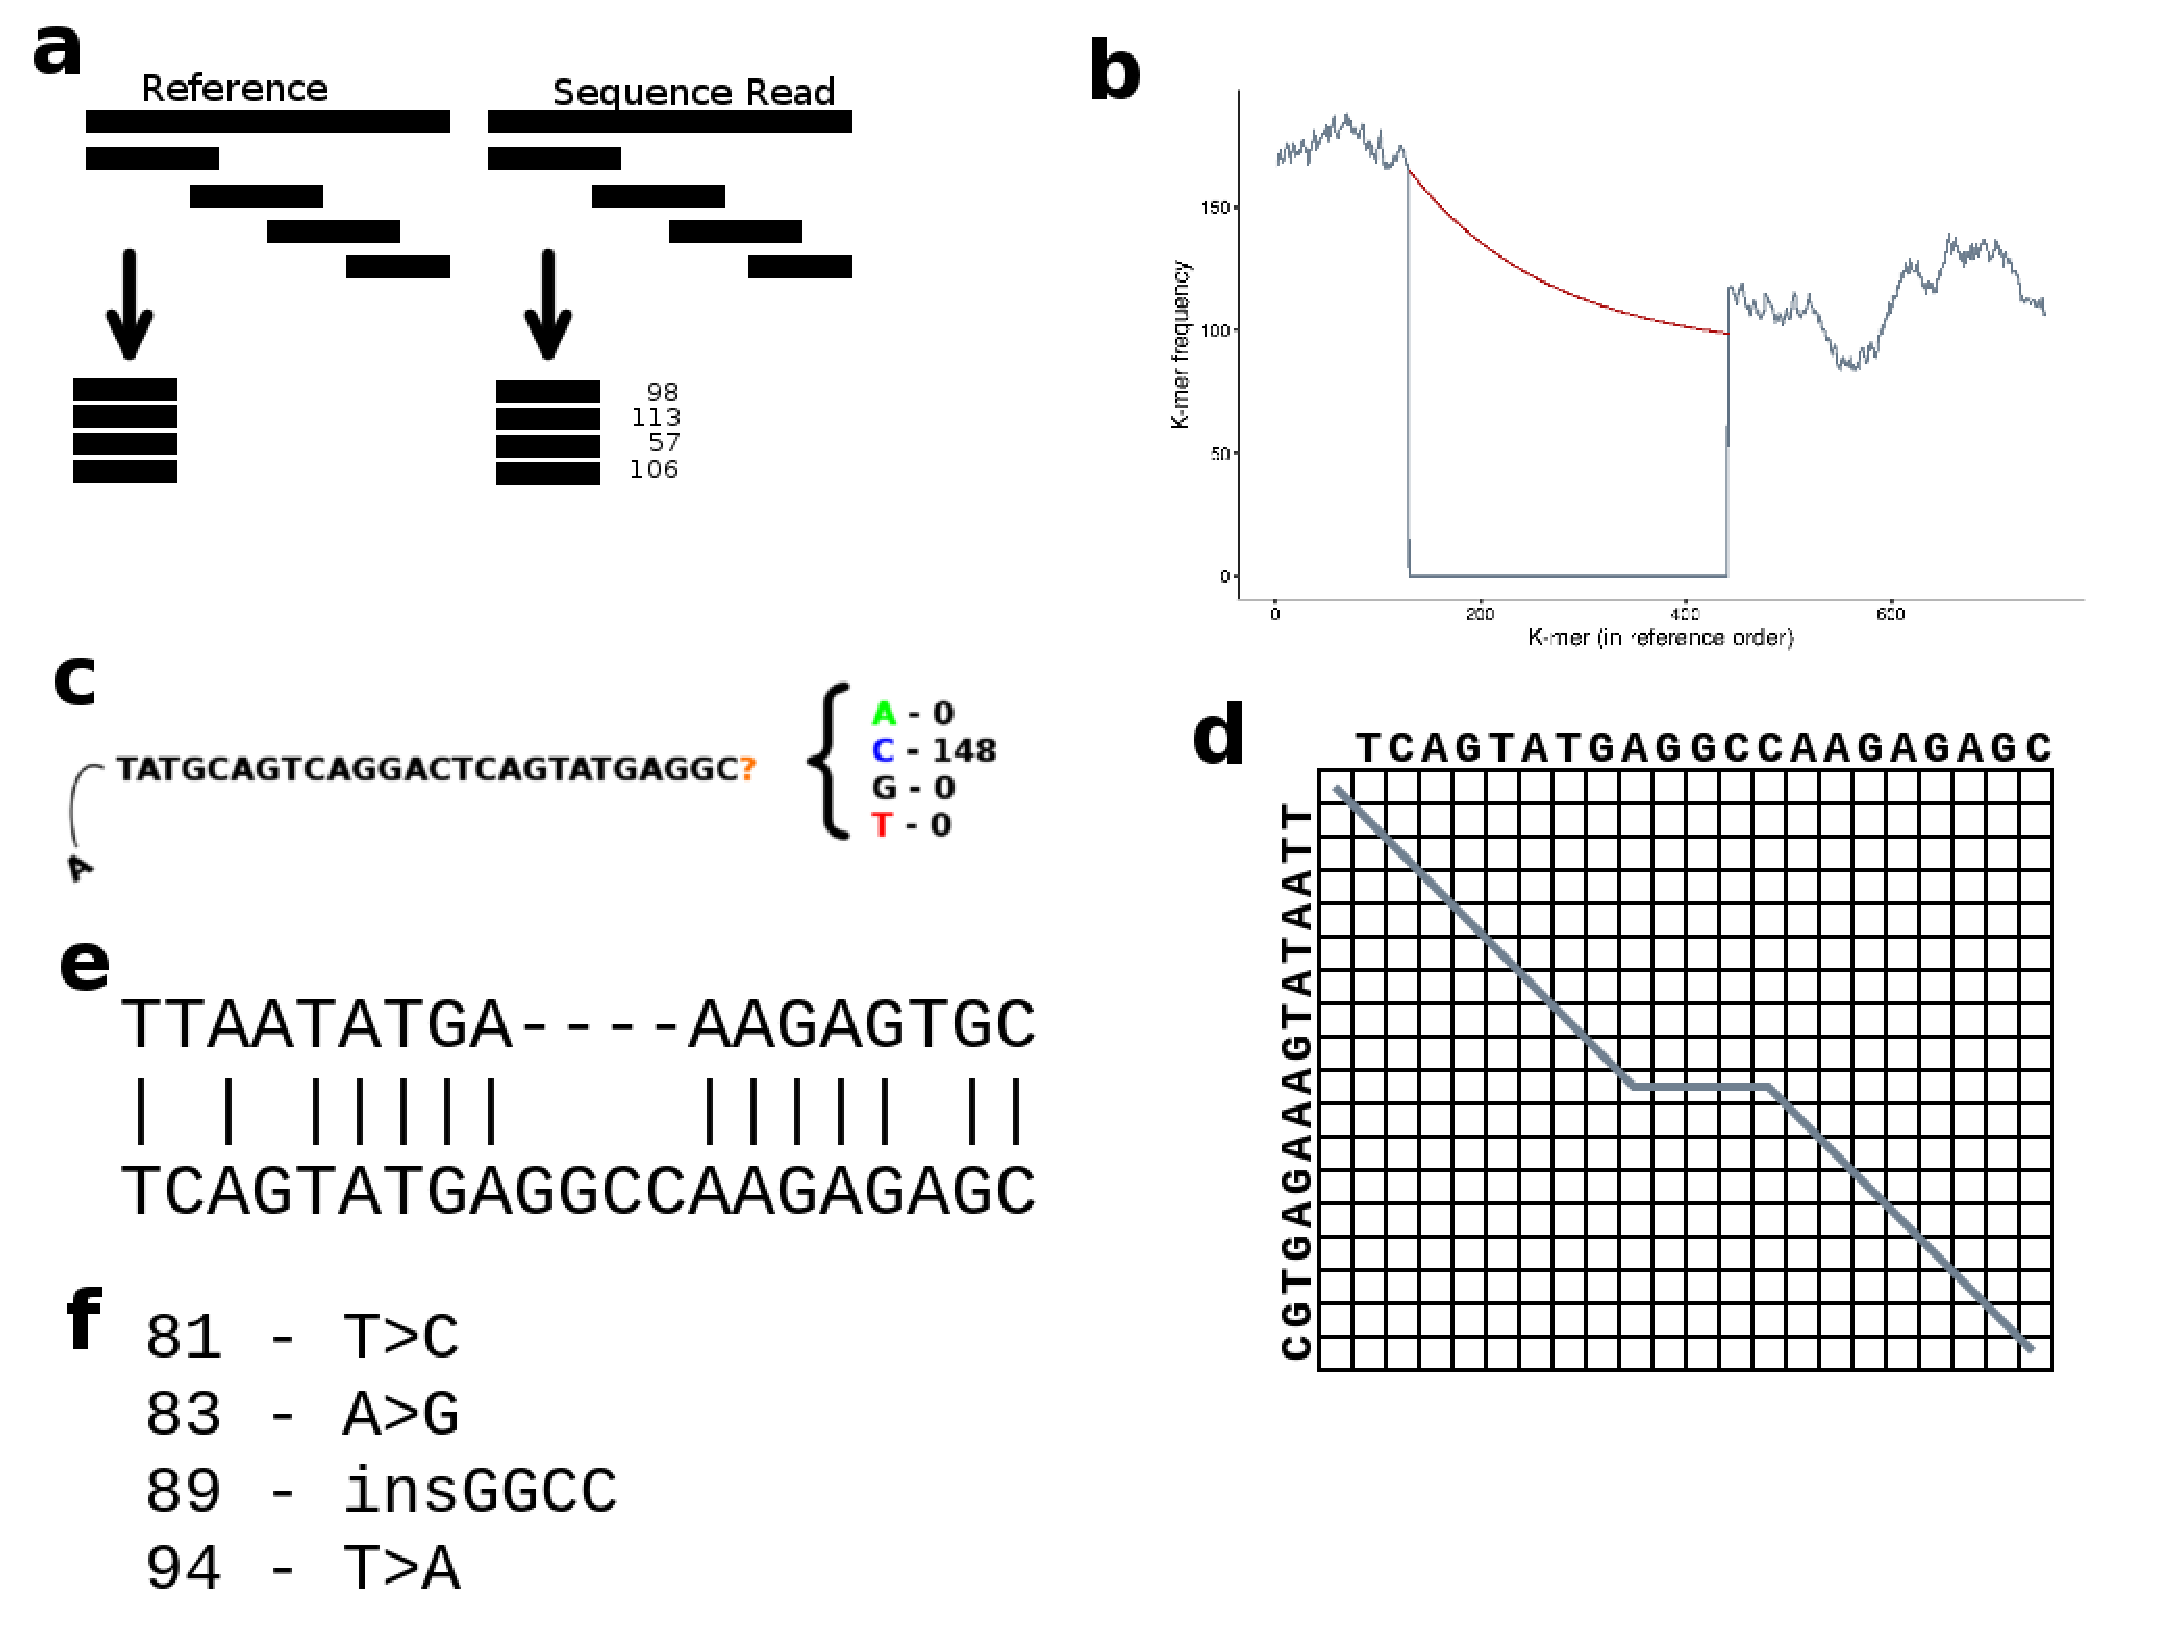
\includegraphics[width=0.75\textwidth]{img/KestrelOverview}
	\end{center}
	
	\caption{Overview of the Kestrel process from sequence data to variant call. \figpart{a} The reference sequence and the sequence reads are converted to k-mers. The k-mers of the sequence reads are counted, but the k-mers of the reference are left in order. \figpart{b} K-mer frequencies from the sequence reads (vertical axis) are assigned to the k-mers of the reference (horizontal axis). A decline and recovery of the frequencies bound an active region where one or more variants are present. \figpart{c} Starting from the left anchor k-mer (last k-mer with a high frequency), the first base is removed, each possible base is appended, and the base that recovers the k-mer frequency is appended to the haplotype. \figpart{d} A modified alignment algorithm tracks haplotype reconstruction and terminates the process when an optimal alignment is reached. \figpart{e} This algorithm yields an alignment of the reference sequence and haplotype within the active region. \figpart{f} Variant calls are extracted from the alignment.}
	
	\label{fig.arillustration}
\end{figure}

Kestrel first translates the reference sequence to a set of ordered k-mers and the sequence reads to k-mer frequencies. The frequency of each reference k-mer and its reverse-complement are queried and examined. The expected distribution of reference k-mer frequencies in a given region is roughly uniform. However, when a variant occurs, the k-mers of the sequence reads differs from the k-mers of the reference, and clear disruptions of the uniform distribution can be observed. For example, a single SNP will change $k$ k-mers, and the frequency of those reference k-mers will be much lower than those around it.

Kestrel scans the list of frequencies from the reference k-mers from left to right searching for regions where it declines sharply and recovers at some downstream k-mer. This region is an \textit{active region} where one or more variants are suspected to be found. The algorithm includes the high-frequency k-mers at either end of the active region, and these are called \textit{anchor k-mers} because the help to seed the process of resolving the region.

Kestrel then builds one or more local assemblies through the active region, and each one is called a \textit{haplotype}. Haplotype reconstruction begins on the left anchor k-mer, and since that k-mer is part of the active region, it is the first $k$ bases of the haplotype. According to active region detection, then next k-mer downstream should be altered, and this fact is used to simplify the process of resolving altered bases using an iterative sliding process.

Starting from the anchor k-mer, the first base is removed, each possible base (A, C, G, and T) are appended to the $(k - 1)$-mer, and the frequency of each possibility is checked. The reverese-complement k-mer is subjected to a similar process, and the frequencies are summed. The base that produces a k-mer with the highest frequency is appended to the haplotype. This process is repeated until the haplotype is fully resolved.

There are a couple of notable exceptions to the the process as described, and these will be covered in more detail. When more than one base produces a k-mer with an acceptable frequency, haplotype reconstruction splits by saving one of the possibilities, building the most likely one, and returning to the other saved states. If a variant occurs too close to the start of a reference, Kestrel can start from the right anchor k-mer and work backwards. In this case, the left anchor k-mer is missing, and a Kestrel option must be used to allow only one anchor.

Kestrel uses a modified Smith-Waterman~\cite{Smith1981} alignment to guide haplotype reconstruction over the active region. When an optimal alignment score is reached, haplotype reconstruction terminates. An additional check ensures that the active region ends on the right anchor k-mer or the haplotype is discarded. If only one haplotype is found and it matches the reference, it is discarded and Kestrel omits nothing for that region.

The alignment of each haplotype over an active region is then used to find variants. Kestrel sums the evidence for the variant from each haplotype it is found in.


\subsection{Input}
\label{sec.process.input}

\subsubsection{Sequence Data}
\label{sec.process.input.seq}
Because Kestrel relies on the KAnalyze~\cite{Audano2014} API for its sequence input, it can take any file format KAnalyze can read. This includes FASTA, FASTQ, gzipped FASTA and FASTQ, and indexed k-mer count (IKC). Kestrel uses the KAnalyze stream mode to convert the reference to an ordered list of k-mers.

\lopt{format} can be used be to force the input file format for all files following it on the command line. The default value, ``auto'', attempts to determine the input file format by the file name. This is handled by KAnalyze, and so Kestrel can input anything KAnalyze can turn into an IKC file. \lopt{stdin} can be used in place of an input file, and Kestrel will read sequence data from standard input.

Sequence data can be filtered before it is turned into k-mers. The options \lopt{seqfilter} and \lopt{quality} are synonymous and equivalent to the KAnalyze sequence filters. The format of the argument to this option is ``FILTER:ARGS'', where FILTER is the filter name, and ARGS is a string of arguments. The format of the arguments is up to the filter, but it is typically a comma-separated string of attributes and values. The default filter is ``sanger'', which applies a quality filter assuming Sanger FASTQ quality scores (Phred scaled). This filter can take a numeric value specifying the minimum score. This option applied the filter to all subsequent input files, but \lopt{noseqfilter} may be used to turn it off so that the filter is not applied to all input.

\subsubsection{Reference}
\label{sec.process.input.seq}

The reference file is input with \lopt{ref}, and this option may be used multiple times if reference sequence is found in multiple files. Reference files are also processed by KAnalyze, and they can be in any format KAnalyze can stream k-mers from (not IKC). The reference does not need to be indexed in any way.

The description line of a FAST record has a sequence identifier with an optional extended description. KAnalyze assumes everything after the first whitespace character is an extended description, and it is not part of the record ID. If whitespace characters are part of the the sequence name and should not be discarded, \lopt{normrefdesc} may be used to retain the description as part of the record ID.


\subsubsection{Samples}
\label{sec.process.input.samples}

Kestrel can call variants on multiple samples in one run, but by default, it assumes all input data belongs to the same sample. Any sample may have more than one file of sequence data in it. These files are read, translated to k-mers, counted, and stored in an IKC file. Any input except IKC file may be mixed into one sample, but if an IKC file is used, it must not be accompanied by any other sequence data including other IKC files.

If no sample names (\lopt{sample}) is given, then Kestrel chooses a name for the sample based on the first input file name. Each time \lopt{sample} is found, it starts a new sample and all subsequent files up to the next \lopt{sample} is grouped into one sample. Samples without any input files are ignored.

In some cases, it is more convenient to input a list of files and have Kestrel separate them automatically instead of repeated used of \lopt{sample}, and Kestrel provides \lopt{filespersample} to make this easier. For example, many samples of paired-end reads can be input by setting \lopt{filespersample} to $2$ and ensuring input files are paired on the command-line. Kestrel will use default names for samples. The default value, $0$, does no automatic grouping. \lopt{sample} will override \lopt{filespersample} and reset the number of files in the current sample if these options are mixed.

\subsection{K-mer Counting}
\label{sec.process.kmers}

The most important option for k-merization is the k-mer size, \lopt{ksize}. Larger k-mers are more specific, but are more likely to contain errors, and fewer k-mers can be extracted from sequence reads. A k-mer size too small is not specific enough, and a k-mer size too large leads to loss of coverage. The default, 31, is used for historical reasons, but k-mers up to size 48 have been used successfully with human data. Tune this parameter for read size and error rate.

Sequence read errors generate erroneous low-frequency k-mers, and \lopt{mincount} controls the minimum frequency. K-mers with a count less than this value will be discarded before being merged into the IKC. This keeps the IKC file to a reasonable size. During k-mer counting, however, all k-mers are written to a temporary location (\lopt{temploc}) before being merged, and the temporary files are automatically deleted.

Input sequence reads are converted to an IKC file. This file is a database of k-mers that can be rapidly searched without loading the k-mer counts into memory. It groups k-mers that likely appear together in a sequence, and when loaded as a memory-mapped file, segments of the file can be loaded as needed. The IKC file is automatically deleted by Kestrel when it is no longer needed, and this can be altered with \lopt{normikc}. KAnalyze can be used directly to generate the IKC in a separate step, and when Kestrel reads an existing IKC, it will never be automatically deleted.

If \lopt{memcount} is set, Kestrel will count k-mers to memory instead of an IKC file. It will be faster to query, but may use an excessive amount of memory.

The IKC format requires that k-mers be grouped by a minimizer, which is defined as the minimum value of all sub-k-mers of a k-mer and its reverse complement. Grouping by minimizers is the key to making IKC files fast without using much memory. The default, and maximum, minimizer size is 15. To better randomize k-mers over low-complexity sequence, minimizers may also be scrambled by an XOR mask by setting \lopt{minmask}. Changing these options is rarely necessary.

Active region detection, haplotype extension, and variant support all use the forward and reverse-complemented k-mers. If an application should strictly analyze and use evidence from a single strand, \lopt{nocountrev} may be set. In most cases, this option would only lower Kestrel's power to detect and resolve variants.

\subsection{Intervals and Flanks}
\label{sec.process.intervals}

Using a BED file specified by \lopt{interval}, Kestrel can call variants in specific regions of the genome. The BED file contains intervals over reference sequences (the first column must match reference sequence IDs).

If each region was treated as a reference sequence, then variants near the ends of the intervals may be lost. Kestrel can extend beyond the edges of these intervals, find active regions, and call variants from the extended interval. Any variants found outside of the actual interval are discarded after calling. By default, Kestrel extends intervals by $1.5 \cdot k$. This behavior can be controlled by \lopt{autoflank}, where a multiple of $k$ is set, or with \lopt{flank} with a set number of bases. Setting either of these options to $0$ will cause Kestrel to not use flanks.

Using intervals gives Kestrel a few output options as well. By default, Kestrel outputs variants relative to the start of the reference sequence, but \lopt{byregion} will output variants relative to the interval the variant was found in. If the BED file contains strand information, \lopt{revregion} may also be set to output variants relative to the positive strand (variants are complemented and shifted accordingly). These options are not recommended for VCF files as they will create a non-standard VCF that other tools and technicians may not know how to interpret correctly.


\subsection{Active Region Detection}
\label{sec.process.ardetect}

For each reference sequence or interval, Kestrel gets the k-mers in the order they appear. It then assigns the frequency from the IKC file to each of the k-mers. Variants between the sample and the reference change k-mers in the sample, and so the k-mers of the reference will have a lower frequency. These frequency disruptions appear as sudden dips followed by a recovery at some downstream k-mer. The active region is defined as the sequence covering these low-frequency k-mers, and it includes the high-frequency k-mers at each end.

\subsubsection{Scan Start}
\label{sec.process.ardetect.start}

The difference between neighboring k-mers must be large enough to trigger an active region scan, and this threshold is set dynamically by Kestrel. First, the difference between each pair of neighboring k-mers is found, and the threshold is set as a quantile of this difference distribution. The default quantile, 0.90, can be set with \lopt{diffq}. According to the default, 90\% of the differences between neighbors will be large enough to trigger an active region scan. This value is rather conservative, but it is limited by \lopt{mindiff} (default $5$), which sets the absolute minimum value this threshold can be regardless of the quantile.

\subsubsection{Scan End}
\label{sec.process.ardetect.end}

An active region scan ends when Kestrel finds an acceptable recovery of k-mer frequency at some downstream k-mer, but since sequence coverage is not uniform, Kestrel must allow for the possibility that the recovery k-mer frequency will be significantly lower than the anchor k-mer frequency where the scan started. Ideally, this threshold would start at the value of the left anchor k-mer and steadily decline to some minimum value as the scan moves further away. This function is defined as $f(x)$ where $x$ is the distance from the anchor k-mer and $f(0)$ is the anchor k-mer frequency.

$f(x)$ is based on a standard exponential decay function, $h(x) = e^{-x \lambda}$, which starts at $1$ and declines steadily toward $0$. $\lambda$ controls how fast it decays. $f(x)$ is defined by shifting $h(x)$ so that it approaches a minimum value, $f_{min}$, and scaled so that it declines from $f(x)$ to $f_{min}$.

Kestrel first determines the minimum value, $f_{min} = f(0) \cdot 0.55$, where the proportion of $f(0)$ can be set with \lopt{decaymin} (default 0.55). The exponential function is then scaled over the remaining distance from $f(0)$ to $f_{min}$ giving $f(x) = (f(0) - f_{min}) \cdot h(x) + f_{min}$.

The last parameter is $\lambda$, which is not set directly. Instead, $\lambda$ is determined by $\alpha$, which is defined as the proportion of $f(0) - f_{min}$ left after $k$ k-mers. The default value of $\alpha$ is $0.80$, and it can be set by \lopt{alpha}. This setting is far more intuitive than choosing some value of $\lambda$, and $\lambda$ can be readily found given $\alpha$ and $k$ (see Kestrel publication for details). Consequently, the range from $f(0) to f_{min}$ declined at $x$ is $x / k \cdot \alpha$. For example, when $X = 3k$, the recovery threshold is $\alpha^3 (f(0) \cdot f_{min}) + f_{min}$.

To summarize, an active region scan starts with anchor k-mer frequency $f(0)$. An exponential decay function is defined, $f(x)$, such that the recovery threshold declines steadily as the distance from the anchor k-mer, $x$, increases. When a k-mer $x$ k-mers away from the anchor is found with a frequency greater or equal to $f(x)$, the scan stops, and the k-mer at $x$ becomes the right anchor k-mer.

It is worth noting that stringently tuning $\alpha$ so that a scan ends at the end of an active region is not usually necessary. It is possible that the scan misses the end of an active region because the read depth declined too quickly. In this case, the active region scan will eventually decline to the read depth and stop. If other variants are nearby, the active region could start over one variant, miss the recovery, go into the next variant, and end when the k-mer frequency recovers. In this example, multiple variants will be covered in one active region, and Kesrel has no trouble with this.

\subsubsection{Resolving the Haplotypes}
\label{sec.process.ardetect.resolve}

When an active region scan successfully ends, the next step is to build haplotypes over it. The active region is then given over to the local assembly process of Kestrel. If at least one variant in the haplotypes exists, then they are output, and the search for the next active region begins after the right anchor k-mer.

If no haplotypes are resolved or if the only haplotype matches the reference, the active region is discarded and the search for the next active region starts from the first k-mer following the left anchor k-mer.

\subsubsection{Peak Detection}
\label{sec.process.ardetect.peak}

The sequence of a genome is not a random distribution of nucleotides. There are patterns, motifs, and duplicated regions, and these can be problematic for k-mer methods. While Kestrel cannot effectively deal with extended regions of homology, it can detect short peaks in the k-mer frequencies and ignore them. The maximum width of a peak in k-mers is set by \lopt{peakscan} (default = $7$). This value is used to avoid starting erroneous active region scans and to avoid prematurely ending active region scans.

When the k-mer frequency increases significantly, Kestrel first looks ahead to see if the frequency quickly declines again. If it does, it jumps ahead to the other side of the peak and continues to search for active regions.

When an active region scan finds a k-mer with a frequency meeting the recovery threshold, it looks ahead by the peak width to see if the frequency declines again, and if it does, it continues the scan from the other side of the peak as if the recovery threshold was not found.

It is possible that the active region scan will find many peaks at the end of an active region when the recovery threshold is very close to the read depth. When several peaks are found in quick succession, the active region scan goes back to the first sharp increase in frequency at the beginning of the peaks and ends there.

\subsubsection{Terminating a Scan}
\label{sec.process.ardetect.terminate}

Some active regions become so large that resolving them with Kestrel would use far too much memory and CPU to resolve, or they may be an erroneous active region. To limit the size of these regions, a limiting factor can be set. The active region limit is defined as the maximum length of a deletion, as calculated using the alignment weights, plus the k-mer size multiplied by $5.0$ (tunable with \lopt{scanlimitfactor}).

Active regions may span ambiguous bases, such as N. If, however, if \lopt{noambiregions} is set and the scan traverses an ambigous base, the active region is discarded.

If an active region reaches the end of the sequence, it cannot have both anchor k-mers and the scan is aborted. See \rsec{sec.process.ardetect.endcalling} for information about relaxing this limitation.

When a scan is terminated, the search for an active region continues from the next k-mer after what was the anchor k-mer in the active region scan.

\subsubsection{End Calling}
\label{sec.process.ardetect.endcalling}

If the active region does not have an anchor k-mer on both ends, it is also discarded by default. To enable calling variants up to the ends of reference sequences, \lopt{noanchorboth} can be set to allow a single anchor k-mer instead of requiring both. Calling to the ends is disabled by default because Kestrel could be extending a haplotype that actually belongs to another region. \lopt{noanchorboth} should be used with caution. For calling variants on intervals, Kestrel uses the flank options (\rsec{sec.process.intervals}) to avoid end-calling.

Kestrel can call variants up to either end of the reference. If a sharp increase of k-mer frequency is found before any other accepted active regions, it suggests that the beginning of the sequence may contain a variant affecting all k-mers at the start of the reference and the high-frequency k-mer is the \textit{right} anchor k-mer. Kestrel can then build from the right anchor k-mer in reverse to resolve variants up to the start of the sequence.

When a region lacks an anchor k-mer, Kestrel also allows deletions at the very ends. For all other regions with two anchor k-mers, end deletions are not allowed because the haplotypes must begin and end with the anchor k-mers.

\subsection{Haplotype Reconstruction}
\label{sec.process.haplo}

Haplotype reconstruction begins with the left anchor k-mer, and it extends to the right anchor k-mer. This process begins by assuming the left anchor k-mer matches the sequence and the haplotype, and so the haplotype sequence is initialized with the anchor k-mer sequence.

\subsubsection{Extending the Haplotype}
\label{sec.process.haplo.extend}

The haplotype is then extended by shifting the k-mer by one base into the active region. This is accomplished by taking the anchor k-mer, removing the left-most base, and appending each possible base (A, C, G, and T) to the $(k - 1)$-mer and seeing which base produces a k-mer with the highest frequency. This base is then appended to the haplotype, and the new k-mer is shifted by the same process to find the next base. This iterative shifting process takes place until haplotype reconstruction is complete.

It is possible that more than one base will produce an acceptable k-mer frequency. Since any k-mer count above $0$ is acceptable, this parameter is tuned by \lopt{mincount}. The base that produces the highest frequency will be appended to the haplotype. Any other base that produces a frequency above $0$ will split haplotype reconstruction. In this case, the state of the current haplotype is saved along with the alternative base. When a haplotype is complete, the first saved state is loaded and its haplotype is completed.

\subsubsection{Haplotype Alignment}
\label{sec.process.haplo.align}

As the haplotype is built, a modified Smith-Waterman alignment algorithm guides the process to avoid spending computing resources on erroneous haplotypes.

Alignment algorithms are driven by a score that is increased when bases match and decreased when bases mismatch or are aligned with a gap (insertion or deletion). Haplotype reconstruction is seeded by the left anchor k-mer, which matches the start of the active region, and so the alignment is initialized by matching all bases along the k-mer. As bases are added to the haplotype, the alignment is updated to include them.

Scores for aligned bases are $R_{match}$ (a positive number) if they match and $R_{mismatch}$ (a negative number) if they do not match. Whenever the alignment transitions into a gap, $R_{open}$ (negative) is added to the score, and $R_{gap}$ ($0$ or negative) is added to the score for each base aligned with the gap (including the first base in the gap). Kestrel also requires that an initial score, $R_{init}$ be set on the alignment, which defaults $k \cdot R_{match}$ since the initial alignment assumes the anchor k-mer, which is $k$ bases long, is unaltered in the sample. These parameters may be tuned with \lopt{weight}.

The alignment proceeds adding each base to the alignment and updating the alignment score appropriately. The highest alignment score is updated as the alignment progresses. Because of the alignment algorithm, Kestrel can also determine when the highest possible alignment score is reached, and this causes haplotype reconstruction to terminate.

The haplotype must end on the right anchor k-mer, and if it does not match every base of the anchor, the haplotype is discarded.

For details about the modified Smith-Waterman algorithm itself, please see Kestrels publications.


\subsubsection{Limiting Haplotype Reconstruction}
\label{sec.process.haplo.limits}

Because haplotypes are constructed from k-mers, they are prone to extend into noise. This is especially true for regions with paralogous k-mers with many other regions or samples with significant contamination. In these cases, Kestrel can spend a great deal of computing resources exploring many haplotypes that often split, and so there are parameters that can keep Kestrel within the confines of the computing environment it runs in.

\rsec{sec.process.haplo.extend} explains how a haplotype can split when more than one k-mer produces an acceptable frequency. This causes Kestrel to save the state of the haplotype at its current place, extend the haplotype with one of the possibilities, and then return to the saved state and extend it for a different possibility. These saved states take memory and CPU time to resolve, and so they can be limited by \lopt{maxalignstates}.

Haplotype states are ordered so that the most likely states will be extended before less likely ones. One haplotype is more likely if it is longer, and if they are equal length, the haplotype with the highest k-mer frequency where it split is extended first. When the limit on alignment states is reached, the least likely haplotype state is discarded first.

It is also possible that many completed haplotypes may be found over an active region, and this too can be limited by \lopt{maxhapstates}.


\subsubsection{End Calling}
\label{sec.process.haplo.ends}

If the the active region goes to the left end of the reference, then the right anchor k-mer seeds haplotype reconstruction. When an active region extends to the end of the reference, there is no anchor k-mer on that side, and so the anchor k-mer restriction is lifted. It also allows deletions up to the end because the end of the reference could have been deleted. While it is possible that some sample may have inserted bases at the ends, Kestrel will never detect it because adding bases to the end of an alignment without downstream matching bases can only lower the alignment score.


\subsection{Variant Calling}
\label{sec.process.varcall}

Variant calling is done directly from the alignments. Mismatched bases are annotated as SNVs, gaps in the reference are insertions, and gaps in the haplotype are deletions. If interval regions are defined and variant calling was done with flanks beyond the region boundaries, then variants on any bases outside of the interval boundaries are discarded.

By default, Kestrel will attempt to resolve all ambiguous bases. Active regions are allowed to cross interval boundaries by default (disable with \lopt{noambiregions}). To allow variants near ambigous bases but to disable variant calls on them directly, \lopt{noambivar} will discard any variants involving an ambiguous reference base.

Variant calls may be filtered by Kestrel with \lopt{varfilter}. Built-in filters include removing variants with low relative depth and filtering by variant type.


\subsection{Output}
\label{sec.process.output}

The default output format is VCF, and this may be set with \lopt{outfmt}. Other built-in types are ``table'' for a parseable tabular format and ``txt'' for a more log-like output. If no output file is set (\lopt{out}), then output goes to standard output (screen).

Assembled haplotypes can also be output with \lopt{hapout}. Kestrel's only built-in format is SAM, but this can be changed using extended libraries (\rsec{sec.process.libs}) and setting \lopt{hapfmt}.

Kestrel has a rich logging infrastructure that can be enabled by setting a log level with \lopt{loglevel}. Valid levels are ALL, TRACE, DEBUG, INFO, WARN, ERROR, and OFF and the names are not case-sensitive. Logs go to standard error by default, but they may be written to a file (\lopt{logfile}) or sent to standard output \lopt{logstdout}.

\subsection{Performance}
\label{sec.process.perf}

Between active regions, Kestrel can free resources it allocated in the aligner instead of reusing them for the next haplotype by setting \lopt{free}. This will never reduce the maximum amount of memory Kestrel uses, but it may reduce the amount of time the memory is consumed. Since Kestrel will have to re-allocate and re-expand arrays in the aligner, this option may have a noticeable performance impact.

\subsection{Extensibility}
\label{sec.process.libs}

Like KAnalyze, Kestrel can be extended and customized by loading external libraries. For example, input and output data could go to a database or some custom file format. Extending Kestrel and KAnalyze is done by writing code that implements a defined interface, compiling it into a JAR file, and then loading the JAR file at runtime. Neither Kestrel nor KAnalyze needs to be modified or recompiled.

Once compiled, these libraries can be loaded from a file (\lopt{lib}) or a URL (\lopt{liburl}). These libraries are shared with the KAnalyze system so that both KAnalyze and Kestrel extensions can be loaded.

\clearpage

%%% Section: API %%%
% Copyright (c) 2017 Peter A. Audano III
% GNU Free Documentation License Version 1.3 or later
% See the file COPYING.DOC for copying conditions.

\section{API}
\label{sec.api}

Kestrel is not only a command line program, it is also an API (Application Programming Interface) that can be driven from other programs. The CLI (Command Line Interface) itself is a simple application that calls the API to carry out tasks.

Kestrel is a Java program, so the API is implemented as a set of Java classes with well documented interfaces. Any Java program can directly call the API classes. Other programs can use technologies such as JNI (Java Native Interfaces) to drive the API from native code, such as C or C++.

Lastly, the command line itself can be used to drive the program from a script or batch file. Because Kestrel always terminates with a well-defined return code, scripts can easily execute the CLI and check for errors. For a list of the return codes, see section~\ref{sec.supl.retcode}.

The remainder of this section outlines the structure and capabilities of the API. It is assumed that a reader of this section has at least a fundamental understanding of Java.


%%%%%%%%%%%%%%%%%%%%%
%%% Documentation %%%
%%%%%%%%%%%%%%%%%%%%%
\subsection{Javadoc Documentation}
\label{sec.api.doc}

The Kestrel API is fully documented with Javadoc comments. Every class and class member (method and field), regardless of scope, has a Javadoc comment. All method arguments, return values, and exceptions are contained in the method's Javadoc comment. For any method arguments that are objects, the comment must disclose what happens when \texttt{null} values are received for that field (either by the argument's comment, or the comment on the exception if one is thrown). All exceptions, whether or not they are runtime exceptions, must be documented along with the conditions that cause them to be thrown. Assertion errors are not documented. Any deviations from these rules should be reported as a program bug.

Javadoc comments can be converted into a set of HTML pages that document the code. In fact, the Java API itself uses Javadoc, so most Java programmers are familiar with the format of the HTML pages. The Kestrel build system will create the Javadoc pages for two different levels: api and full. The API level contains only public and protected members, while the full documentation contains everything. For a programmer interested in using the API or creating a custom component, the API level documentation is probably sufficient. The full documentation is intended for maintenance programmers.

For more information on building Javadoc HTML pages from source, see section~\ref{sec.suppl.building.javadoc}.


%%%%%%%%%%%%%%%%%%%%
%%% Organization %%%
%%%%%%%%%%%%%%%%%%%%
\subsection{Project Organization}
\label{sec.suppl.organization}



%%%%%%%%%%%%%%%%%%%%%%%
%%% Utility Classes %%%
%%%%%%%%%%%%%%%%%%%%%%%
\subsection{Utility Classes}
\label{sec.api.util}

Kestrel has several utility classes for shared functionality. Most of the classes are used by multiple components or modules. These classes may also be useful for other applications.

All of these classes are found in package \texttt{edu.gatech.kestrel.util}

%%% BoundedQueue %%%
\subsubsection{InfoUtil}
\label{sec.api.util.infoutil}


\clearpage

%%% Section: Implementation %%%
% Copyright (c) 2017 Peter A. Audano III
% GNU Free Documentation License Version 1.3 or later
% See the file COPYING.DOC for copying conditions.

\section{Implementation Details}
\label{sec.impl}

This section contains important implementation details for those wishing to extend or maintain Kestrel.

\subsection{Condition Reporting System}
\label{sec.impl.conditions}

TODO: Fill in this section.

\clearpage

%%% Section: Supplementary Information %%%
% Copyright (c) 2017 Peter A. Audano III
% GNU Free Documentation License Version 1.3 or later
% See the file COPYING.DOC for copying conditions.

\section{Supplementary Information}
\label{sec.suppl}


%%%%%%%%%%%%%%%%%%%%%%%%%%%%%%%%%
%%% Command Line Return Codes %%%
%%%%%%%%%%%%%%%%%%%%%%%%%%%%%%%%%
\subsection{Command Line Return Codes}
\label{sec.supl.retcode}

The KAnalyze user interface always returns a well-defined code. When executed from a script environment, this return code can easily be checked to see if KAnalyze completed normally or not. Each return code is defined in this section.

In the following list of return codes, the numeric code is listed. For API users, the constant defined in \texttt{edu.gatech.kanalyze.Constants} is also
listed.

\begin{description}
\item[0 (ERR\_NONE)] The program terminated normally. All k-mers were successfully processed without error, or the help option was invoked.

\item[1 (ERR\_USAGE)] Command line arguments were incomplete, improperly formatted, or required arguments were missing.

\item[2 (ERR\_IO)] An I/O (input/output) error occurred reading or writing data. This error is normally returned for file I/O errors.

\item[3 ERR\_SECURITY] A security error, such as permissions denied, occurred.

\item[4 (ERR\_FILENOTFOUND)] A required or specified file was not found.

\item[5 (ERR\_DATAFORMAT)] Data in an input file is improperly formatted. 

\item[6 (ERR\_ANALYSIS)] Some un-recoverable error occurred during analysis.

\item[7 (ERR\_INTERRUPTED)] A program thread was interrupted while it was running. This would normally be returned if the program is terminated before it completes.

\item[8 (ERR\_LIMITS)] A limitation was reached that forced the program to terminate. This should only occur in extreme cases and may indicate an problem with the input. For example, if more than $2^{63}$ sequences are in a FASTA file, it will trigger this error.

\item[98 (ERR\_ABORT)] The program or a process was terminated before it completed. When the action is requested or expected, this should be returned in lieu of ERR\_INTERRUPTED even if interrupting threads was necessary.

\item[99 (ERR\_SYSTEM)] Some serious unrecoverable system error occurred. These errors are almost certainly program bugs. Some other unrecoverable errors, such as running out of memory, could return this code.

\end{description}


%%%%%%%%%%%%%%%%%%%%%%%%%%%%
%%% Building From Source %%%
%%%%%%%%%%%%%%%%%%%%%%%%%%%%
\subsection{Building From Source}
\label{sec.suppl.building}

The source is distributed with an Apache Ant build file with multiple targets. To build these, Apache Ant must be installed.

To run a target, enter \texttt{ant <target>}. Multiple targets may be supplied, for example \texttt{ant clean package}.

The most commonly used targets are ``clean'', ``compile'', and ``package''. The clean removes all temporary files. It is not often necessary, but it should be executed before building a package for testing to ensure no artifacts are left behind from previous builds. The compile target compiles the class files and does nothing else. The package target generates the JAR file and distributable packages.

The ``doc.javadoc'' target generates the Javadoc pages from Kestrel source comments. See Section~\ref{sec.suppl.building.javadoc} for more information about these pages. ``doc.manual'' generates this manual as a PDF file.

Other targets are called by the targets described above and are not often called directly.

For a full list of targets and brief descriptions, enter \texttt{ant -projecthelp}.


%%%%%%%%%%%%%%%%%%%%%%%%%%%%%%
%%% Building Javadoc Pages %%%
%%%%%%%%%%%%%%%%%%%%%%%%%%%%%%
\subsubsection{Building Javadoc Pages}
\label{sec.suppl.building.javadoc}

Javadoc is a very powerful tool for documenting APIs written in Java. Section~\ref{sec.api.doc} introduces the concept and the KAnalyze rules governing these comments.

Javadoc comments begin with ``/**'', and end with ``*/''. In Kestrel, these comments appear before every class, method, and field. The comment starts with a description of what the element does. For methods, it documents parameters and the conditions under which all exceptions are thrown. Full documentation for writing these comments can be found online\footnote{http://www.oracle.com/technetwork/java/javase/documentation/index-137868.html}. 

The ant build system (Section~\ref{sec.suppl.building}) generates web pages from these comments. The ``doc.javadoc'' target builds two sets of pages. One, the API documentation, documents all elements available on the API. This target is intended for developers who are extending or using the API. The other, FULL documentation, documents everything including private members that are not available to the API. This is meant for Kestrel maintenance programmers.

After running the javadoc Ant target, the API documentation can be access by loading ``build/doc/javadoc/api/index.html'' in a browser (relative to the project root). The FULL documentation can be access by loading ``build/doc/javadoc/full/index.html'' in a browser (relative to the project root).

\clearpage

%%% Section: License %%%
% Copyright (c) 2017 Peter A. Audano III
% GNU Free Documentation License Version 1.3 or later
% See the file COPYING.DOC for copying conditions.

\section{License}
\label{section:license}

% Documentation License %
\subsection{Documetation}

This document is licensed under the GNU Free Documentation License 1.3 or later. The file ``COPYING.DOC'' contains the text of this license. If you did not receive the file in the source distribution, please contact us or the GNU website for a copy.


% Software License %
\subsection{KAnalyze Software}

The Kestrel software is licensed under the GNU Lesser General Public License version 3 or later. The file ``COPYING'' contains the text of the GNU GPL, and the file ``COPYING.LESSER'' contains the GNU LGPL extension to the GPL. If you did not receive the file in the source distribution, please contact us or the GNU website for a copy.

\clearpage

%%%%%%%%%%%%%%%%%%
%%% References %%%
%%%%%%%%%%%%%%%%%%
\bibliography{main}

\end{document}
